\section{Information Architecture}
If we talk about User Centred Design and modern day solutions, one of the most important thing is ``Information Architecture". It is the feature which clearly indicates the quality of the product, UCD is so crucial that extremely complex algorithms are designed to focus on the user needs and to focus on type of the user. It may take several iterations to create a presentable information architecture. In order to match high degree of usability the focus is very deep on the information architecture. It is the feature that helps navigate the complete product without any serious effort or without consuming much time. A good information architecture has property that users can quickly understand what the navigation says. Its very crucial to use easy and meaningful navigation in order to have quality information architecture and pleaseant usability experience. ~\cite{informationIA}\par
Embold has also an easy to explore information architecture, there is relevant information about various components, features and their functionalities.  If    we have a look on general navigation bar of Embold website and Embold tool, it has quite reasonable navigation bar. Website has the horizontal navigation bar as shown in Figure ~\ref{fig:horizontal}, and it contains a very detailed information about the tool, price plans, enterprise categories and much more. A user can easily understand as it's a good usability experience, user centred design and quality standards are kept into the mind while designing.\par
\begin{figure}[htbp]
\begin{center}
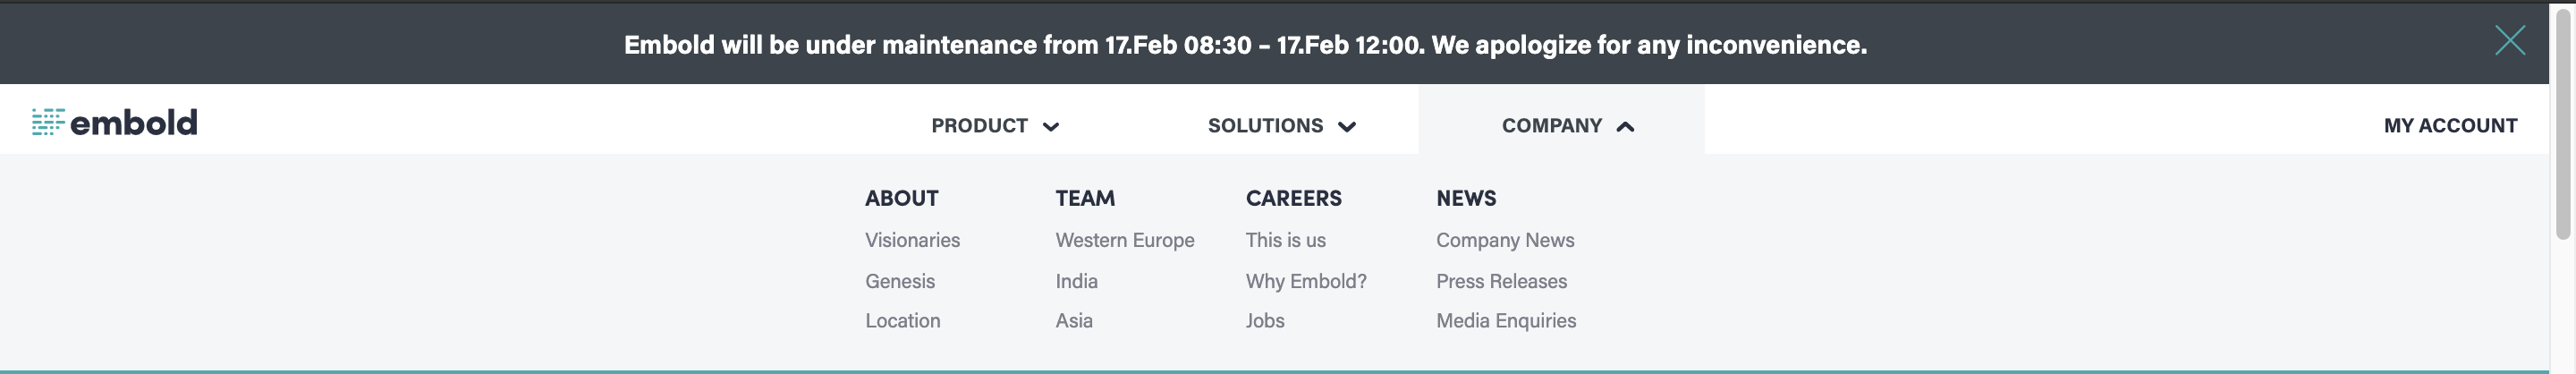
\includegraphics[width=6.5 in, height=1.7in]{Horizontal.png}
\caption{Horizontal Website Navigation ~\cite{emboldio}}
\label{fig:horizontal}
\end{center}
\end{figure}

\indent Now if we look into dashboard navigation or navigation of the Embold Tool as shown in the Figure ~\ref{fig:vertical}.  It looks acceptable. As still there is a room of the improvement. There could be detail information about the projects and other activities. But overall the information architecture is simple, easy to understand, it is hierarchal, logical and tag based. \par
If we talk about in depth Information Architecture is not actually UX Design, but a good Information Architecture leads a user for better UX Design and usability experience. Information architecture is based on the nature of the website and the content of the website. It truly depends on the product, the design team has to change the information architecture as per user needs considering a lot of things. Famous Information Architects Rosenfeld and Peter Morville mentioned in their book ``Information Architecture for the World Wide Web" that Information Architecture has four main components i.e 
\begin{itemize}
\item\emph{Organization Systems:}The approach used to categorize, classify and structure the available content .
\item\emph{Labelling Systems:} The approach of presenting the information which we have. 
\item\emph{Navigation Systems:}  The approach to move through the information, how to use identifiers in order to reach to a specific stage or to get a specific data.
\item\emph{Searching Systems:} The approach which enable users to search for their desired information. 
\end{itemize} 
If we need to understand and develop the successful Information Architecture, it is necessary to understand the user, their context of use and the content available. Because at the end we have to cluster all the data depending on the user needs and the way he thinks or works. ~\cite{IA} \par
So it is same for the  Embold, a user will look for the type of the plan available for the Enterprises. Also if we move towards the further task related activity, a user has ease to select the repository from his version. Also a user gets the detailed information about his code analysis. So the information is classified in categories and presented in a significant manner.\par
If we talk about the navigation system of Embold, it carries a lot of information which sometimes is not very much required. It does not have highlighting effect which can help us to differentiate the various identifiers in the navigation. Also there is the room  for the improvement in the fonts.  The navigation bar also does not include the most required features about search etc. We can not differentiate which is the navigation bar and which on is the information bar as shown in ~\ref{fig:vertical}. \par
While good thing about the navigation bar is that it provides some good information about the tool and it also lands us to the new page if we want to log in to the code analyzer. It also uses information bar to update us about all the changes, updates or any news related to Embold which is quite comprehensive.
\begin{figure}[htbp]
\begin{center}
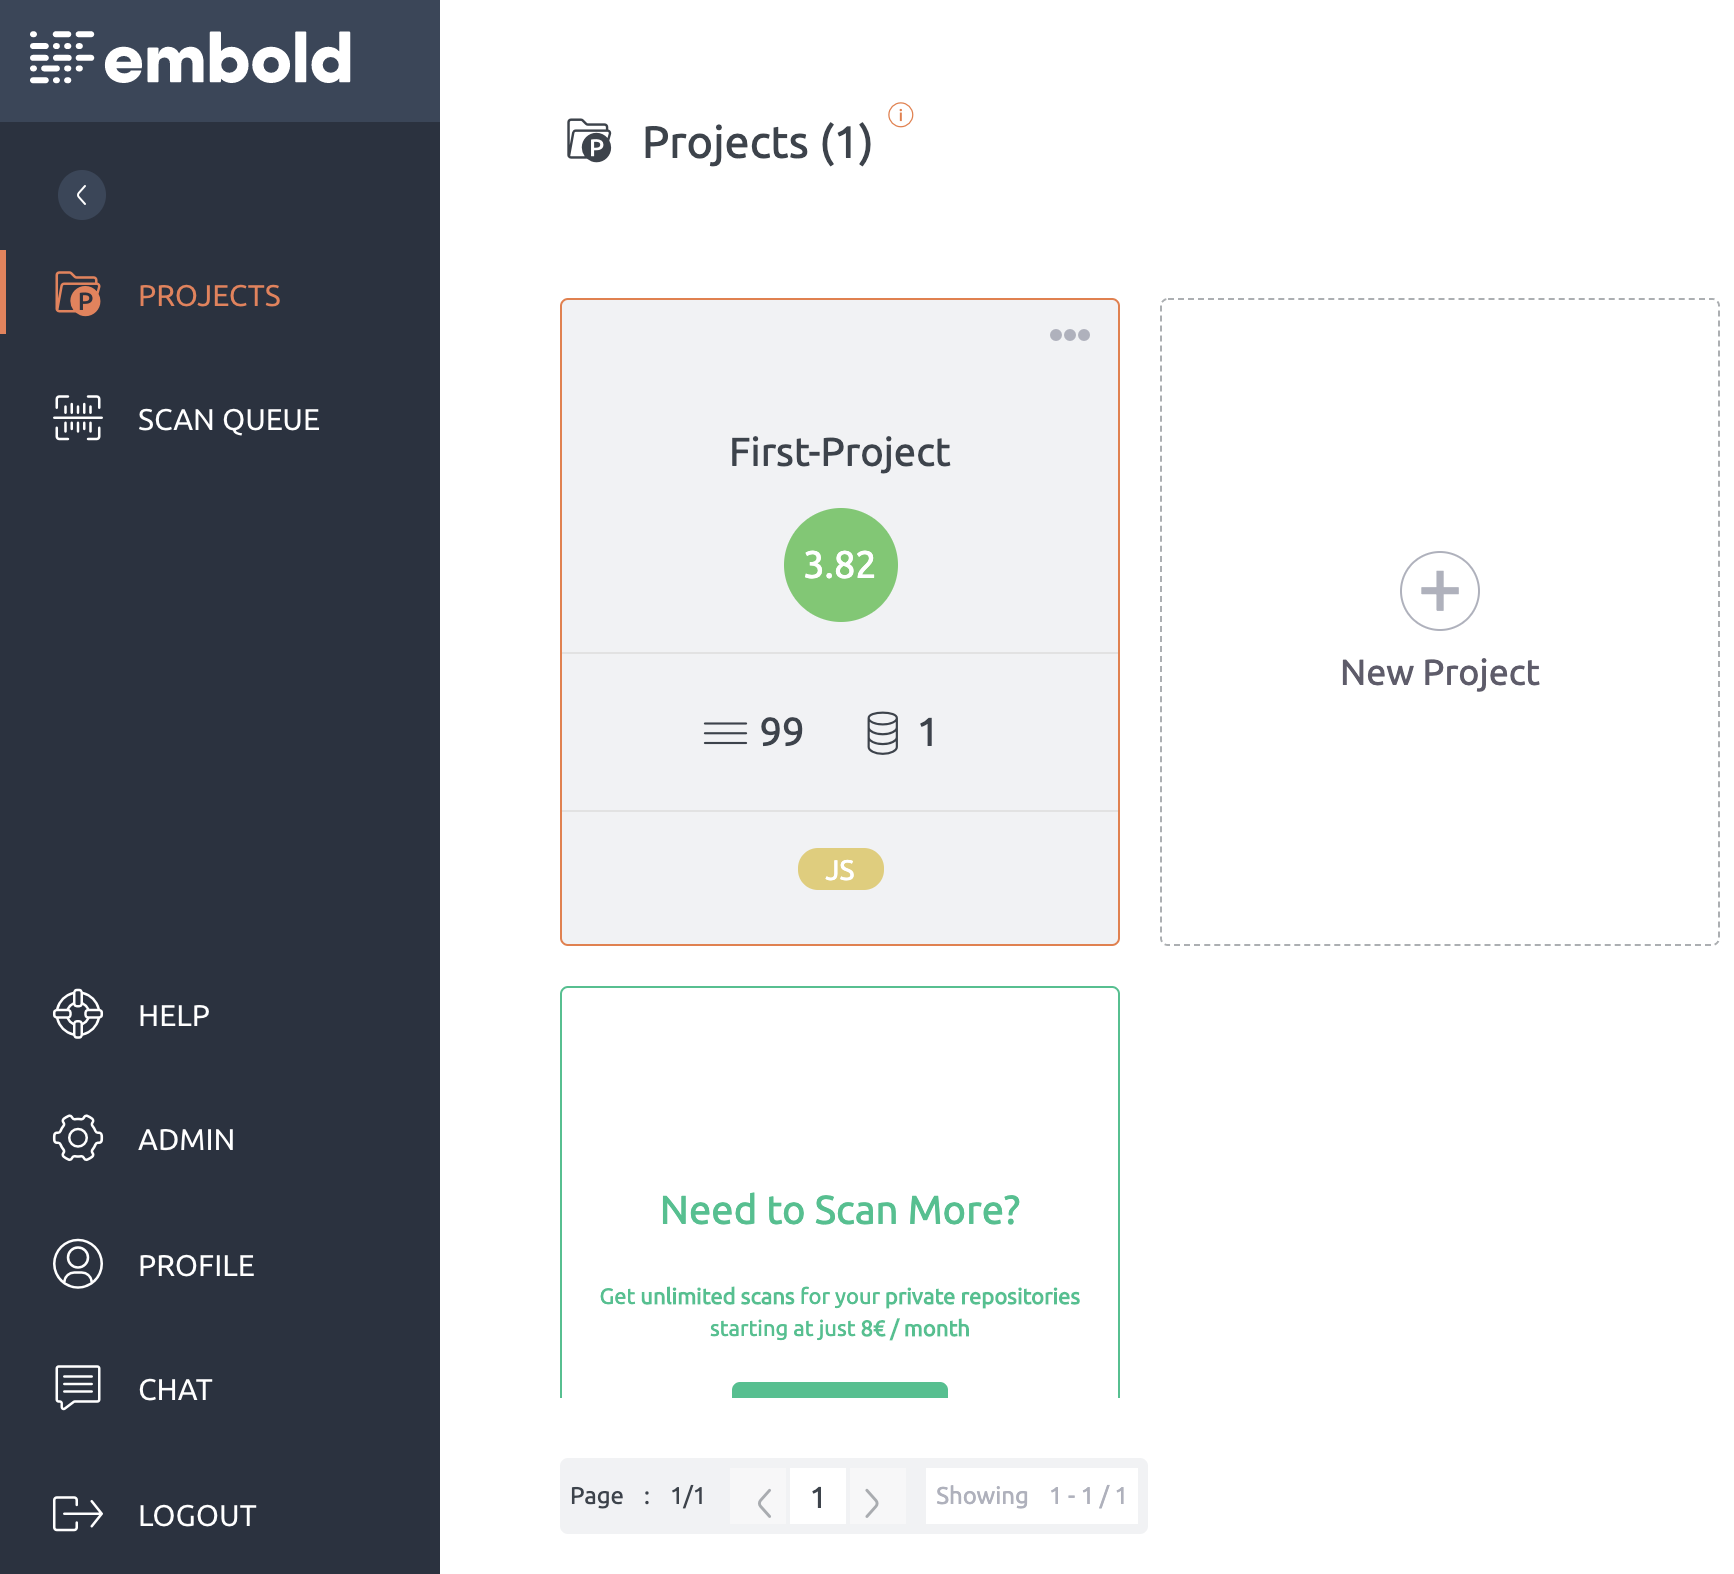
\includegraphics[width=6.5 in, height=3 in]{vertical.png}
\caption{Vertical Navigation Embold Analyzer ~\cite{emboldio}} 
\label{fig:vertical}
\end{center}
\end{figure}

\section{Style Guide - Comparison with ISO 9241-210}
Style Guide or UI style guide is somewhat the display of any solution and it is make or break feature of any product. Style Guide is an artifact of the design process and it  is created to bring together the Designer and Developer on the same page. It is very important for the successful production. Style guide is created by the UX designer. Before preparing a style guide it is important to classify the components of the style guide and have a clear idea what components merge to form a style guide. The figure ~\ref {fig:style}  explains the overview of a style guide. It contains the information about the text style sizes used in the design. \par
\begin{figure}[htbp]
\begin{center}
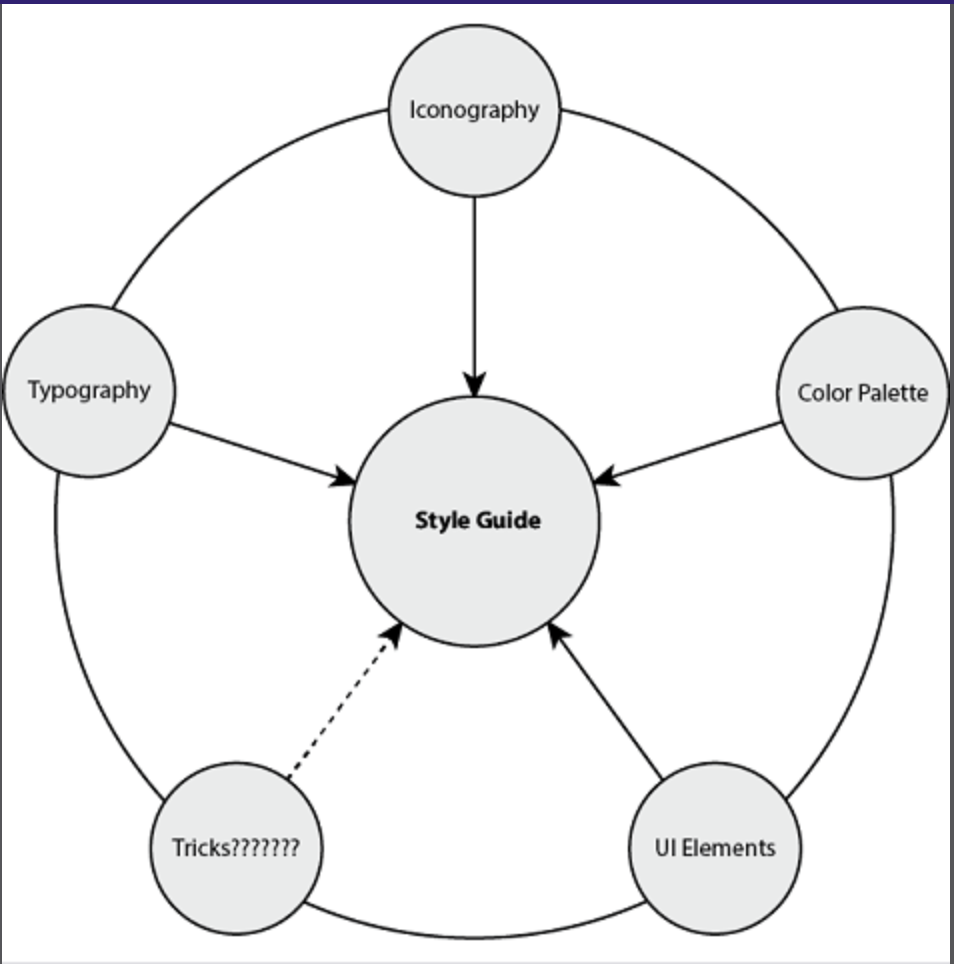
\includegraphics[width=4 in, height=3 in]{style.png}
\caption{Components of a Style Guide~\cite{sguide}}
\label{fig:style}
\end{center}
\end{figure}
Style guide gives an accurate information about the colour codes, size of the buttons, form types, icons types and many other things which eventually help the developer in order to be on the same page with designer. All the User Interface (UI) designs have a style guide, UI is prepared considering the ISO standards about Human Centred Design and mainly User Centred Design.  SO it is very important to understand the ISO standards to produce a better product. Most of the times it's the UI  which pushes new users and explore the product more, in many cases users purchase the premium package just because of the UI design when they are at par with other products of the same UX Design.  So UI could be a tie breaker in few situations. \par
\subsection{ISO 9241-210}
If we talk about ISO Standard 9241:210, Human Centred Design for interactive systems; there are clear guidelines to develop useful and useable products. The scope of ISO 9241-210 is towards all of the design processes where both the hardware and software components of interaction systems can be used to enhance the Human System interaction.\par
The useful and usable products with better UX experience are developed by keeping in mind the user needs, user requirements and  HCD guidelines defined in ISO standards.
\begin{figure}[htbp]
\begin{center}
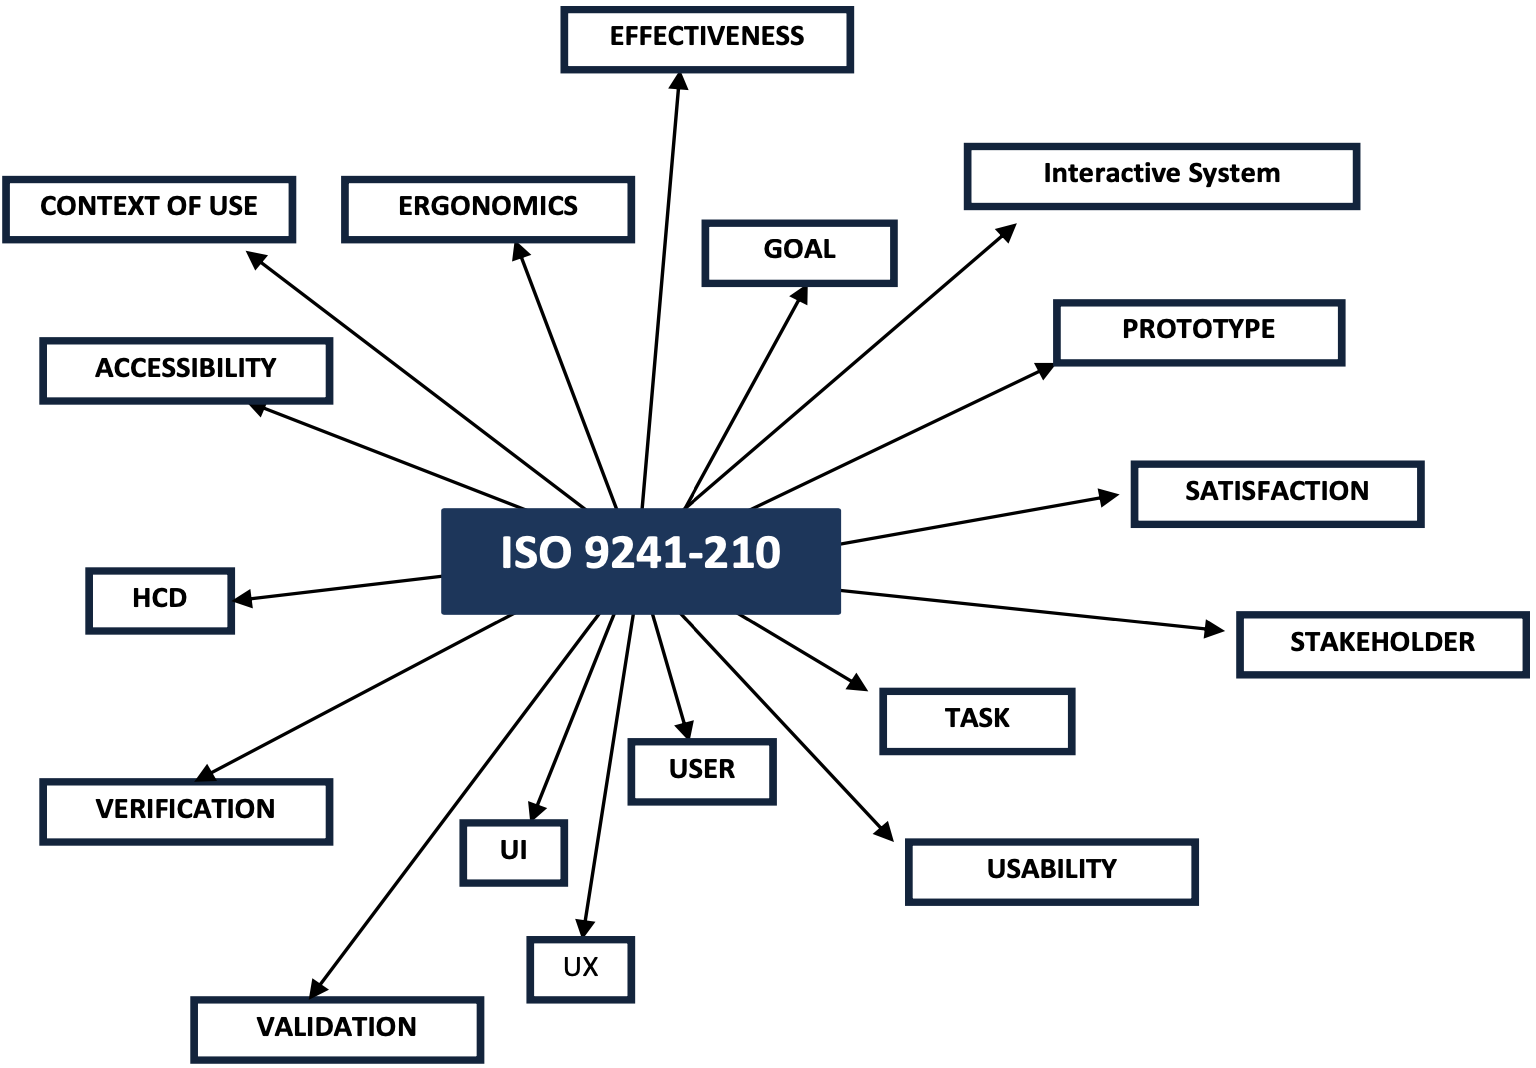
\includegraphics[width=4 in, height=3 in]{ISO.png}
\caption{ISO 9241-210 Features ~\cite{features}}
\label{fig:ISO}
\end{center}
\end{figure}
If we see the Figure ~\ref{fig:ISO} we can have a generic overview that what the ISO standard 9241-210 ~\cite{ISO} is about. It clearly defines a variety of aspects, whether it's about the user, user context, quality of the tool, functionality, tasks, goals and many other aspects. So before preparing any product is very helpful to consider all these aspects, which eventually help to yield in a very handy product. If I draw a comparison with Embold with these ISO standard, we can see a variety of aspects from Embold which will validate those features defined in ISO standards. For example a user is clearly defined, that someone with the Version Control Repository, and it validates before analyzing the code that the code which is being tested is coming from the version control. 
It comes up with specific goal, showing the various kind of results with a variety of descriptions available about the code quality, code issues, hot spots and duplication.  \par
A better UX is there as well, moving through the dash board is a seamless experience, a comprehensive logging in feature is available which moves quickly to the Embold dash board. 
If we talk about UI experience, it is not up-to the mark, as there is no clear difference between signifiers while hovering over them. The colour combination and schemes are not that which attract users. It is not as bad but still something which is below par to the standard. 
As Embold is a code analyzer, so it gives us option to add a variety of programming languages. It also comes up with many results which can help different user groups. It validates many aspects from ISO standard 9241-210, as it is being developed keeping in mind the needs of different users. Like a developer would love to see his progress, project managers would get a knowledge about the risks, potential delays and many other aspects, while the software architects get the actual design issues and all that with the progress of the real time project. \par
It is clearly as per ISO standards, that a user can the Embold according to his condition and requirement, a user can integrate it to any of the development environment. So overall user experience is up-to the mark which makes the Embold a useable and useful product. \par
While considering about user and their requirements, when a user will think about using Embold they will expect a good and readable out-look; they expect it to be easily access able. A user will expect the Embold to be compatible with the modern version control systems, they expect it to be available in various packages related to price and availability. They also expect it to provide information about bottlenecks, road blocks, quality of the software and also help about the estimation of finance and length of the project. \par
Now if we say that whether the Embold has meet up the use expectations, its not very difficult to answer as it has meet up the expectations as far as functionality and security is concerned. While there is room for improvement  in the design, display and outlook.  
